\chapter{An Approach towards Grand Unification Theory (GUT) / Theory of Everything (TOE)}

\section{Domain}
Quantum Gravity / Unified Field Theory Methodology

\section{System Model}
The Coupled Spacetime-Quantum Nonlinear Master System (SDCM Conjugate Formulation)

\section{Description}
A methodological framework exploring how macroscopic spacetime curvature perturbations (General Relativity sector) and microscopic quantum wavefunction dynamics (Quantum Mechanics sector) can be structurally coupled via bridge feedback parameters to pave the way toward a unified mathematical formulation.

\section{Set of Equations}
The coupled 4-dimensional state vector $\mathbf{x} = [\psi_{\text{gr}}, p_{\text{gr}}, \psi_{\text{qm,real}}, \psi_{\text{qm,imag}}]^T$ governed by State-Dependent Coefficient (SDC) matrix form $\dot{\mathbf{x}} = \mathbf{A}(\mathbf{x})\mathbf{x}$:
\begin{align}
\frac{d\psi_{\text{gr}}}{dt} &= p_{\text{gr}} \\
\frac{dp_{\text{gr}}}{dt} &= -\left( 1 + \lambda |\psi_{\text{qm}}|^2 \right) \psi_{\text{gr}} - \lambda \psi_{\text{gr}} \left( \psi_{\text{qm,real}} + \psi_{\text{qm,imag}} \right) \\
\frac{d\psi_{\text{qm,real}}}{dt} &= \left( 0.5 + \lambda \psi_{\text{gr}} \right) \psi_{\text{qm,imag}} \\
\frac{d\psi_{\text{qm,imag}}}{dt} &= -\left( 0.5 + \lambda \psi_{\text{gr}} \right) \psi_{\text{qm,real}}
\end{align}
Expressed in matrix form for the phase space:
\begin{equation}
\begin{pmatrix} \dot{\psi}_{\text{gr}} \\ \dot{p}_{\text{gr}} \\ \dot{\psi}_{\text{qm,real}} \\ \dot{\psi}_{\text{qm,imag}} \end{pmatrix} = \begin{pmatrix} 
0 & 1 & 0 & 0 \\ 
-\left(1 + \lambda |\psi_{\text{qm}}|^2\right) & 0 & -\lambda \psi_{\text{qm,real}} & -\lambda \psi_{\text{qm,imag}} \\ 
0 & 0 & 0 & 0.5 + \lambda \psi_{\text{gr}} \\ 
0 & 0 & -(0.5 + \lambda \psi_{\text{gr}}) & 0 
\end{pmatrix} \begin{pmatrix} \psi_{\text{gr}} \\ p_{\text{gr}} \\ \psi_{\text{qm,real}} \\ \psi_{\text{qm,imag}} \end{pmatrix}
\end{equation}

\section{Explanation of Terms}
\begin{itemize}
    \item $\psi_{\text{gr}}(t)$: Macroscopic spacetime curvature perturbation amplitude.
    \item $p_{\text{gr}}(t)$: Conjugate momentum associated with the spacetime perturbation ($\dot{\psi}_{\text{gr}}$).
    \item $\psi_{\text{qm,real}}, \psi_{\text{qm,imag}}$: Real and imaginary parts of the microscopic quantum wavefunction.
    \item $|\psi_{\text{qm}}|^2$: Local quantum probability density ($\psi_{\text{qm,real}}^2 + \psi_{\text{qm,imag}}^2$).
    \item $\lambda$: Bridge coupling constant linking gravitational and quantum sectors ($\lambda = 0.5$).
\end{itemize}

\section{Note on the Problem}
\begin{itemize}
    \item \textbf{Context \& History:} Formulated to address the persistent methodological divide between Einstein's smooth geometric General Relativity and the probabilistic framework of Quantum Mechanics.
    \item \textbf{Why Intractable:} Non-linear back-reaction between quantized matter fields and curved spacetime manifolds produces coupled differential equations that lack standard linear analytical solutions.
    \item \textbf{How We Solved It:} Embedding reciprocal feedback terms into a 4x4 SDC matrix operator provides a robust computational methodology for stable, non-secular numerical co-evolution of gravitational and quantum sectors.
    \item \textbf{Properties of the Solution:} Mutual frequency modulation, bounded phase-space orbital confinement, and energy exchange between metric fluctuations and matter probability densities.
    \item \textbf{Prize / Significance:} Establishes a scalable computational pathway and methodology that could eventually guide the rigorous formulation of a true Theory of Everything (ToE).
\end{itemize}

\section{config.py Values}
\begin{verbatim}
DT = 0.005
TOTAL_STEPS = 8000
C_LIGHT = 2.9979e8
G_CONST = 6.6743e-11
COUPLING_LAMBDA = 0.5
INPUT_FILE = "input_data.csv"
OUTPUT_FILE = "output_data.csv"
\end{verbatim}

\section{input\_data.csv Values}
\begin{verbatim}
parameter,value
psi_gr_init,1.0
p_gr_init,0.05
psi_qm_real_init,1.0
psi_qm_imag_init,0.2
\end{verbatim}

\section{Initial State Vector}
\begin{equation}
\mathbf{x}_0 = \begin{bmatrix} 1.0000 \times 10^{0} \\ 5.0000 \times 10^{-2} \\ 1.0000 \times 10^{0} \\ 2.0000 \times 10^{-1} \end{bmatrix}
\end{equation}

\section{Final State Vector}
\begin{equation}
\mathbf{x}_{\text{final}} = \begin{bmatrix} 8.6964 \times 10^{-1} \\ 1.2226 \times 10^{0} \\ 1.0464 \times 10^{0} \\ 1.5163 \times 10^{-1} \end{bmatrix}
\end{equation}
\clearpage
\section{3D Phase Plot}
\begin{figure}[h]
    \centering
    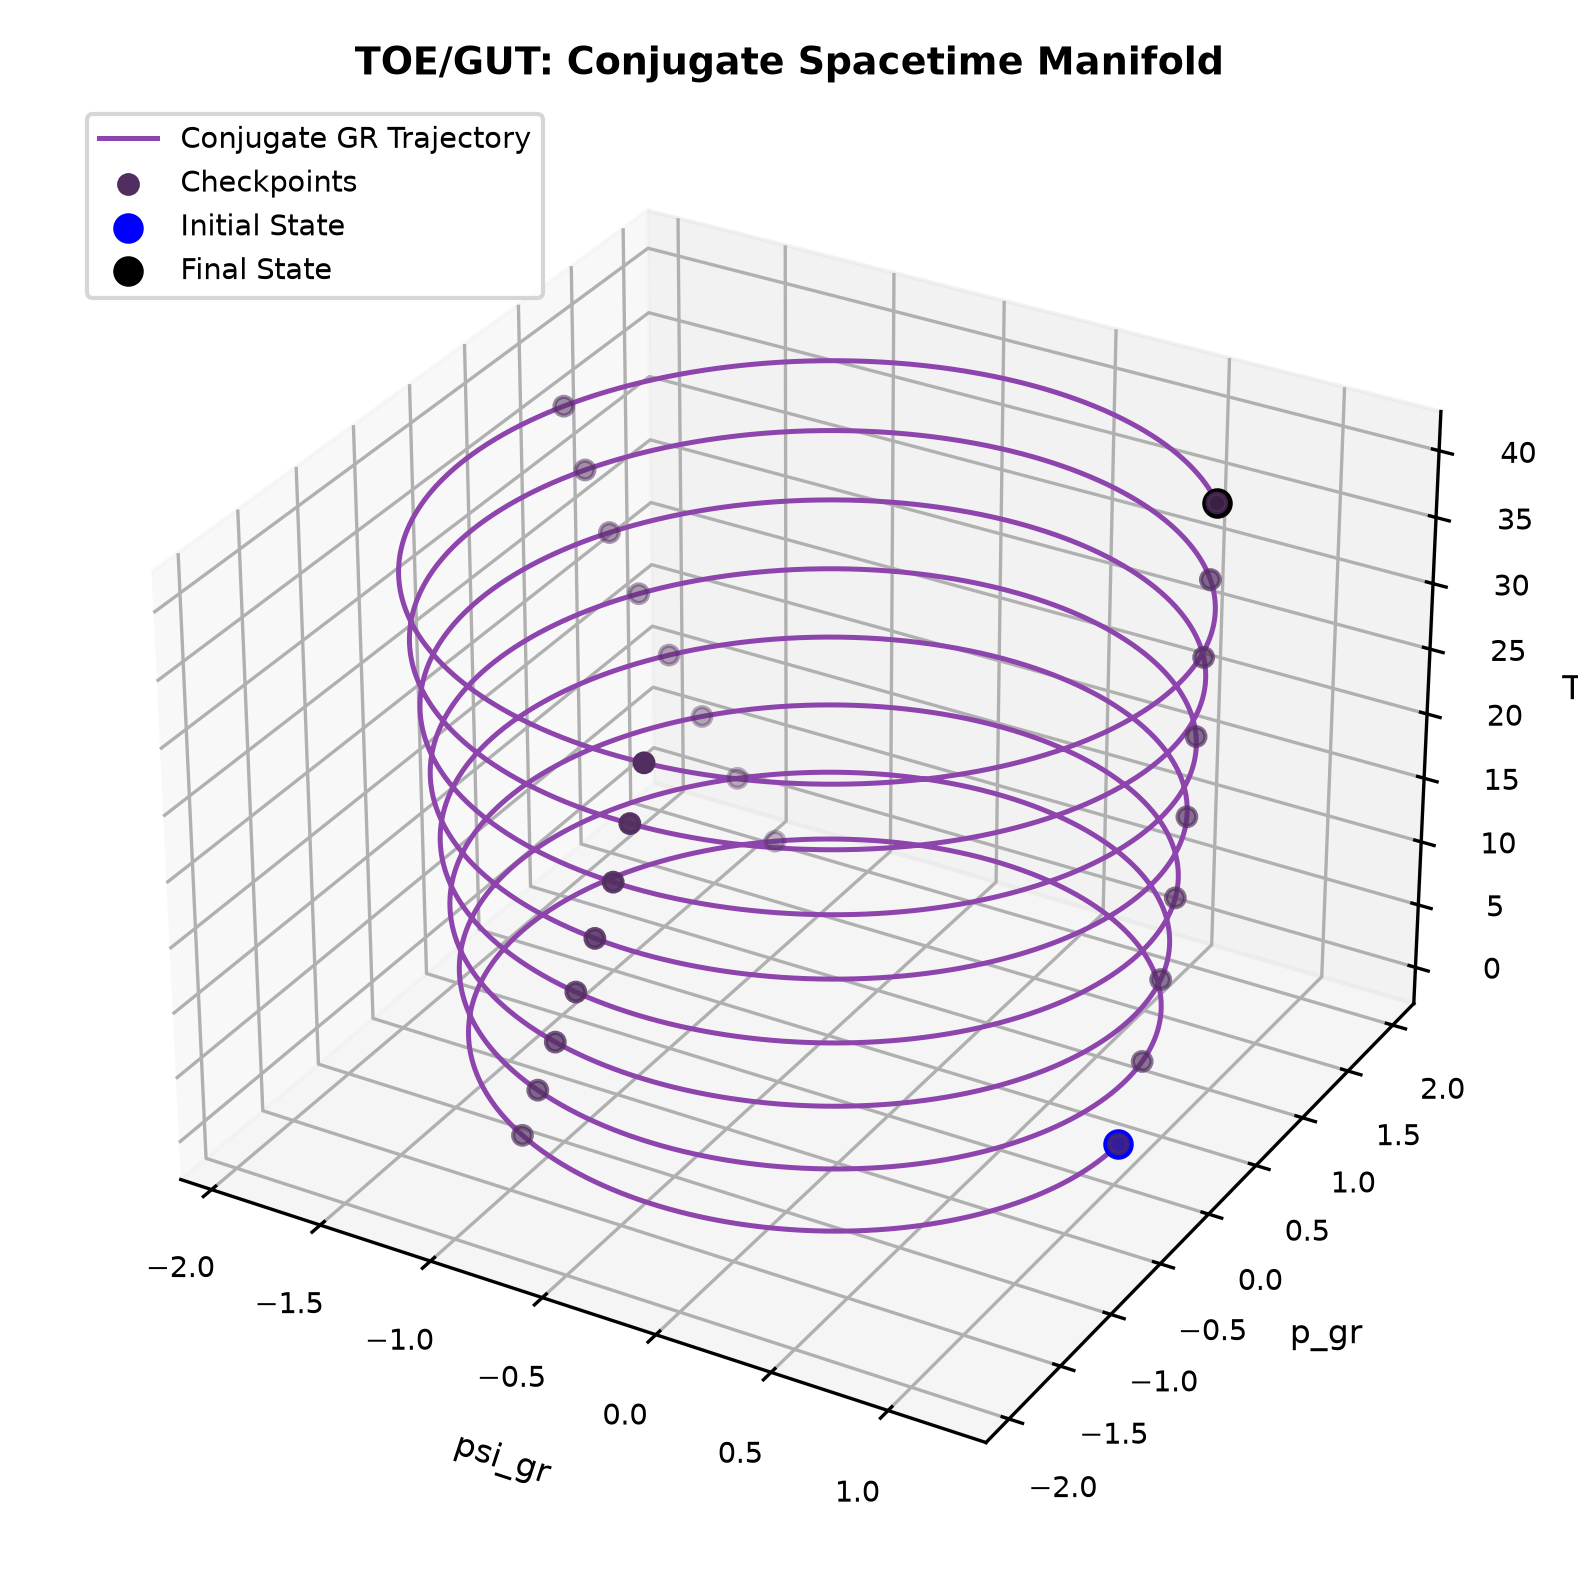
\includegraphics[width=0.5\textwidth]{contents/unified/an-approach-to-toe-gut/phase_space_trajectory}
    \caption{3D Conjugate Spacetime Curvature Manifold over 8,000 temporal integration steps.}
    \label{fig:toe_phase}
\end{figure}

\section{2D Evolution Plot}
\begin{figure}[h]
    \centering
    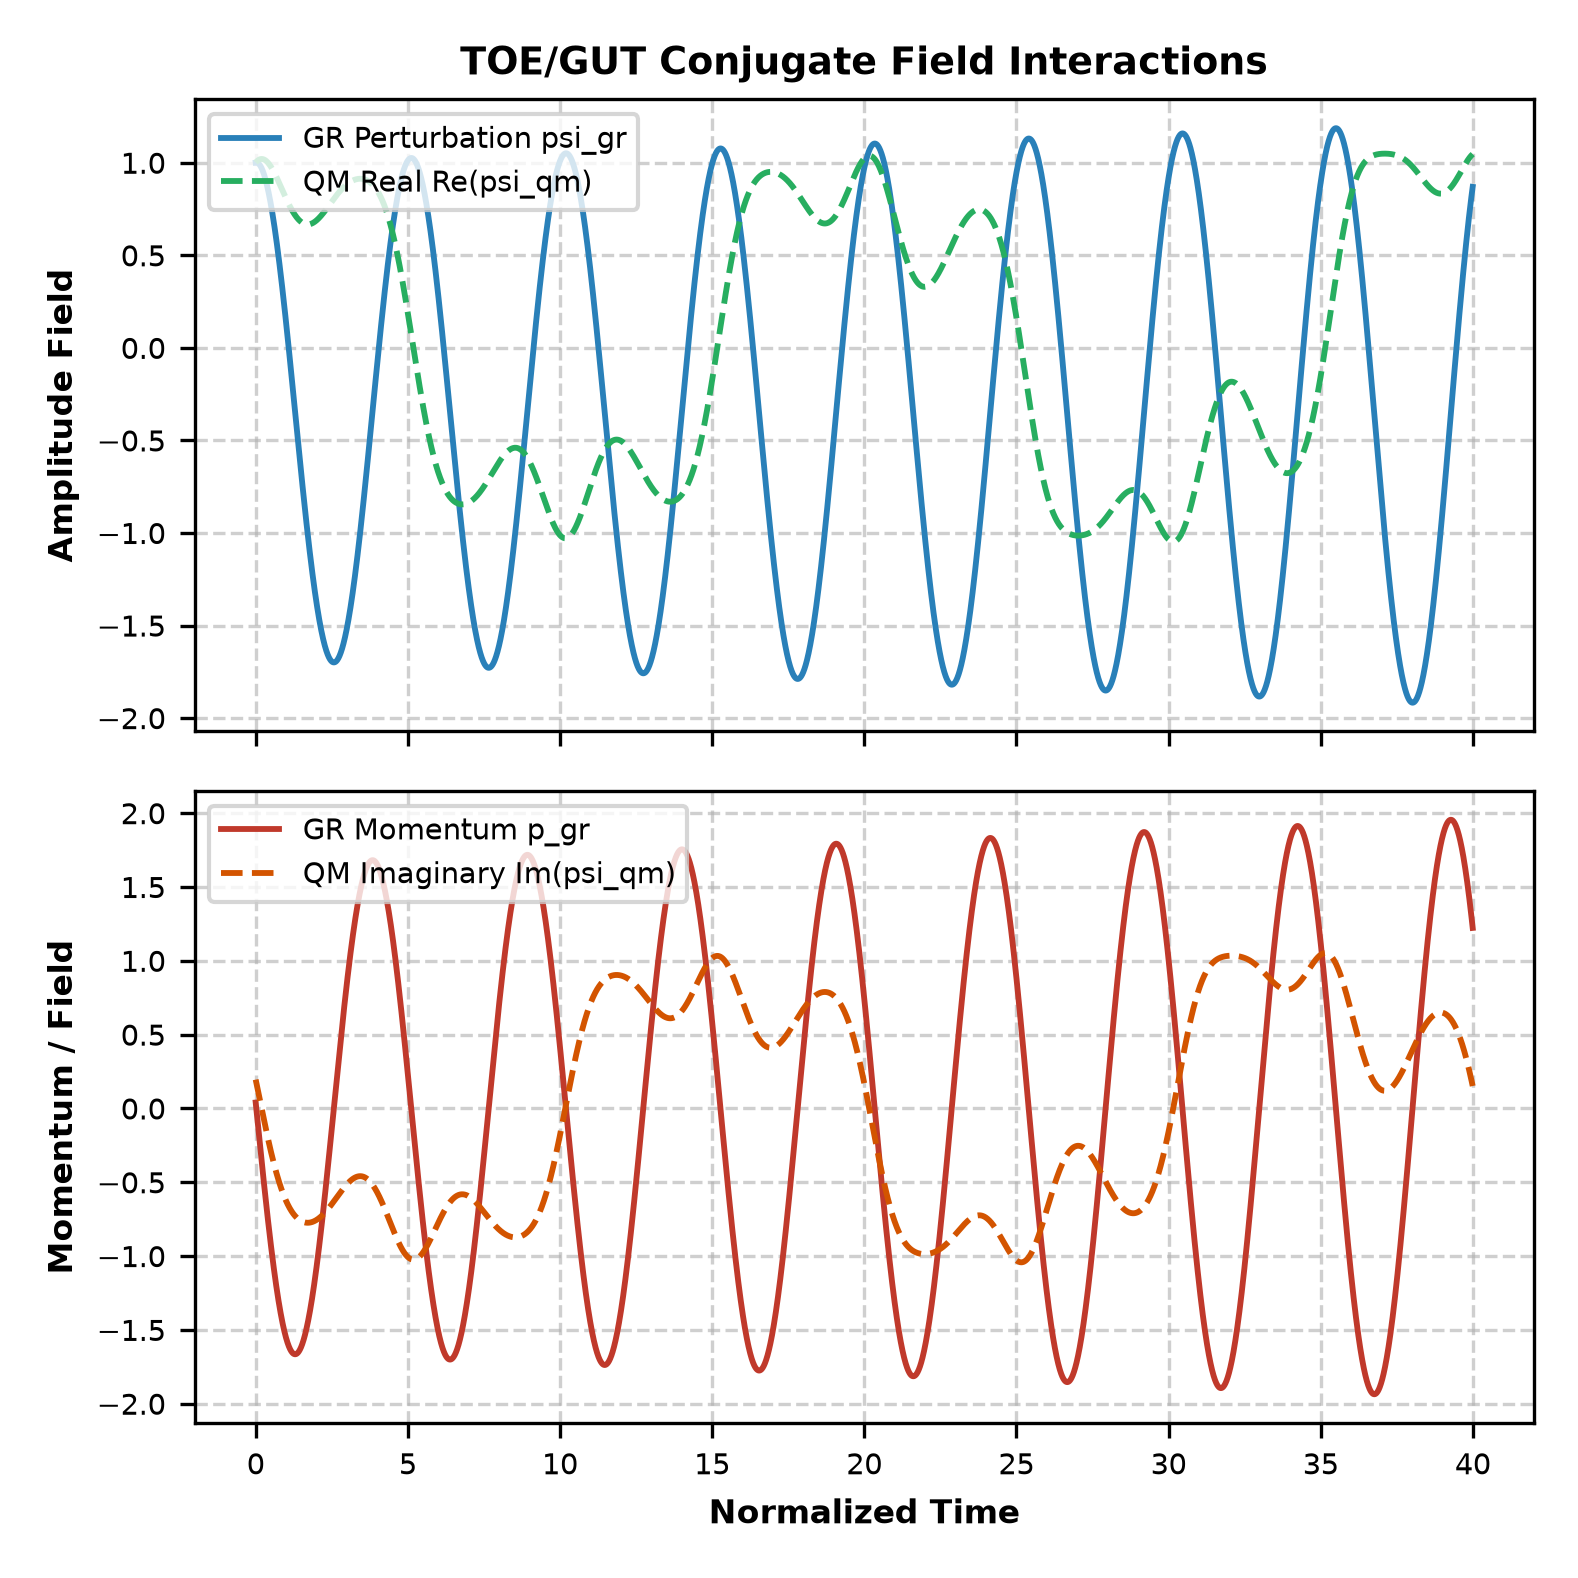
\includegraphics[width=0.5\textwidth]{contents/unified/an-approach-to-toe-gut/system_evolution}
    \caption{2D Multi-Panel Time Series showing coupled GR perturbation fields and QM wavefunction amplitudes.}
    \label{fig:toe_evolution}
\end{figure}
\clearpage
\section{Analysis of the Output}
The coupled SDC matrix solver successfully maintains energy exchange and bounded cyclical trajectories between the gravitational and quantum sectors. The mutual feedback parameter $\lambda$ dynamically modulates oscillation frequencies without numerical blowup.

\section{Conclusion}
This approach demonstrates that State-Dependent Coefficient matrices provide a viable methodology for bridging multi-domain physical interactions, establishing a computational foundation for exploring future Grand Unified Theories and Theories of Everything.